\section{What Makes A Good Mesh}

In general, there are four different parameters that drive the meshing process.

\toIndex{mesh type}
We can specify the mesh type -- the simple geometric differential we'd like to use to model the core with, like tetrahedrals (triangular pyramids) and hexahedrons (rectangular prisms).

\begin{didyouknow}
All other parameters equal, it always takes more tetrahedrons to mesh a model than hexahedrons.  While this means that it has the potential to be better for analyisis than a hexahedral mesh, it also means that it takes more computer resources -- like memory or disk space -- to store or manipulate a tetrahedral mesh.
\end{didyouknow}

\toIndex{axial mesh size}
\toIndex{mesh size!axial}
Additionally, we can control how many layers tall we want the mesh to be.  We specify this by setting the axial mesh size, which is the unit length of each mesh layer in the vertical direction.  For example, a core that is 100 units high with an axial mesh size of 20 would produce 5 layers down the side of the mesh.  If you were to change the axial mesh size to 50, two layers would be seen down the sdie.  As with mesh type, a core must have the same axial mesh size in order to be conforming.

\begin{figure}[H]
	\begin{center}
		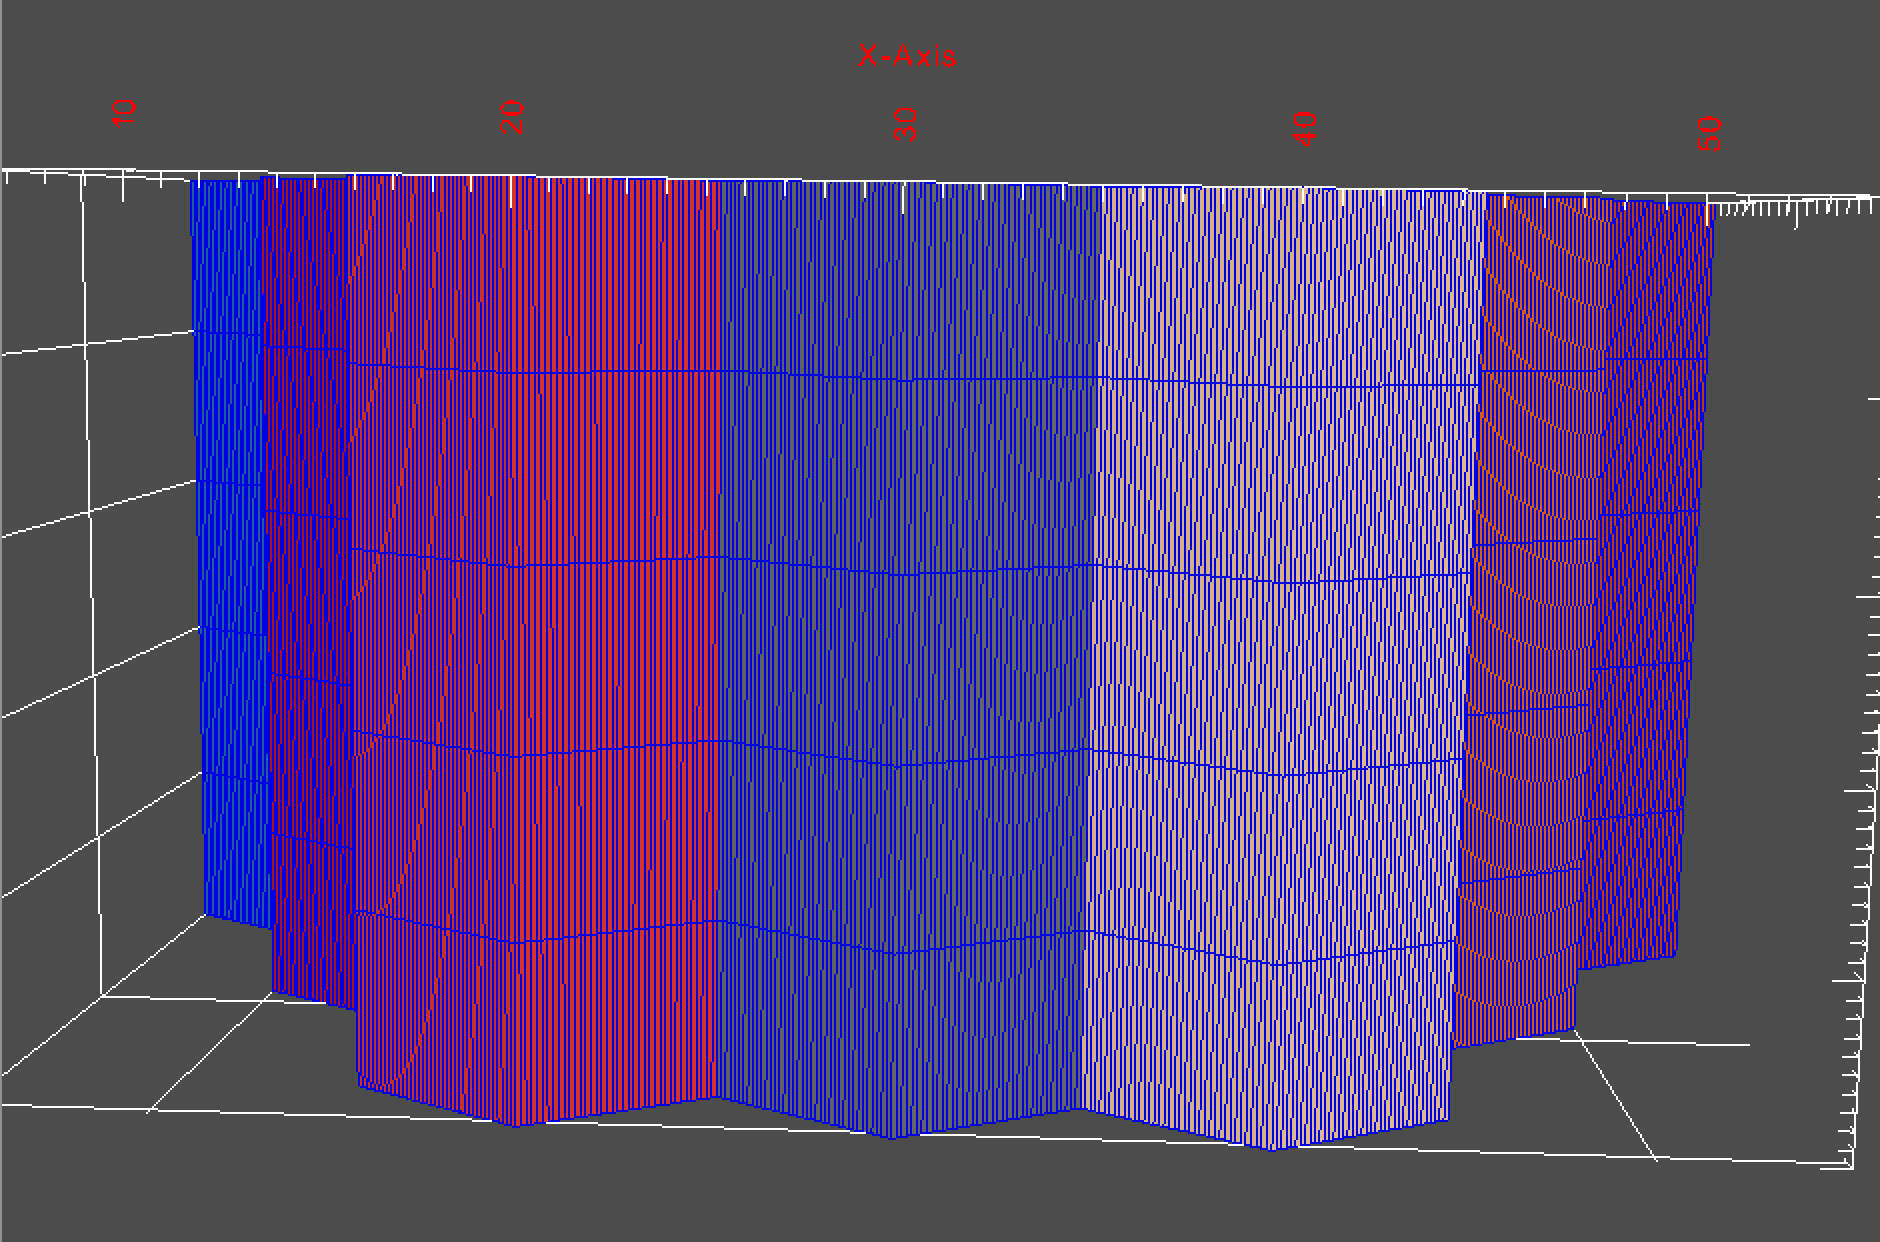
\includegraphics[width=0.5\linewidth]{Images/axial-mesh-20.png}
		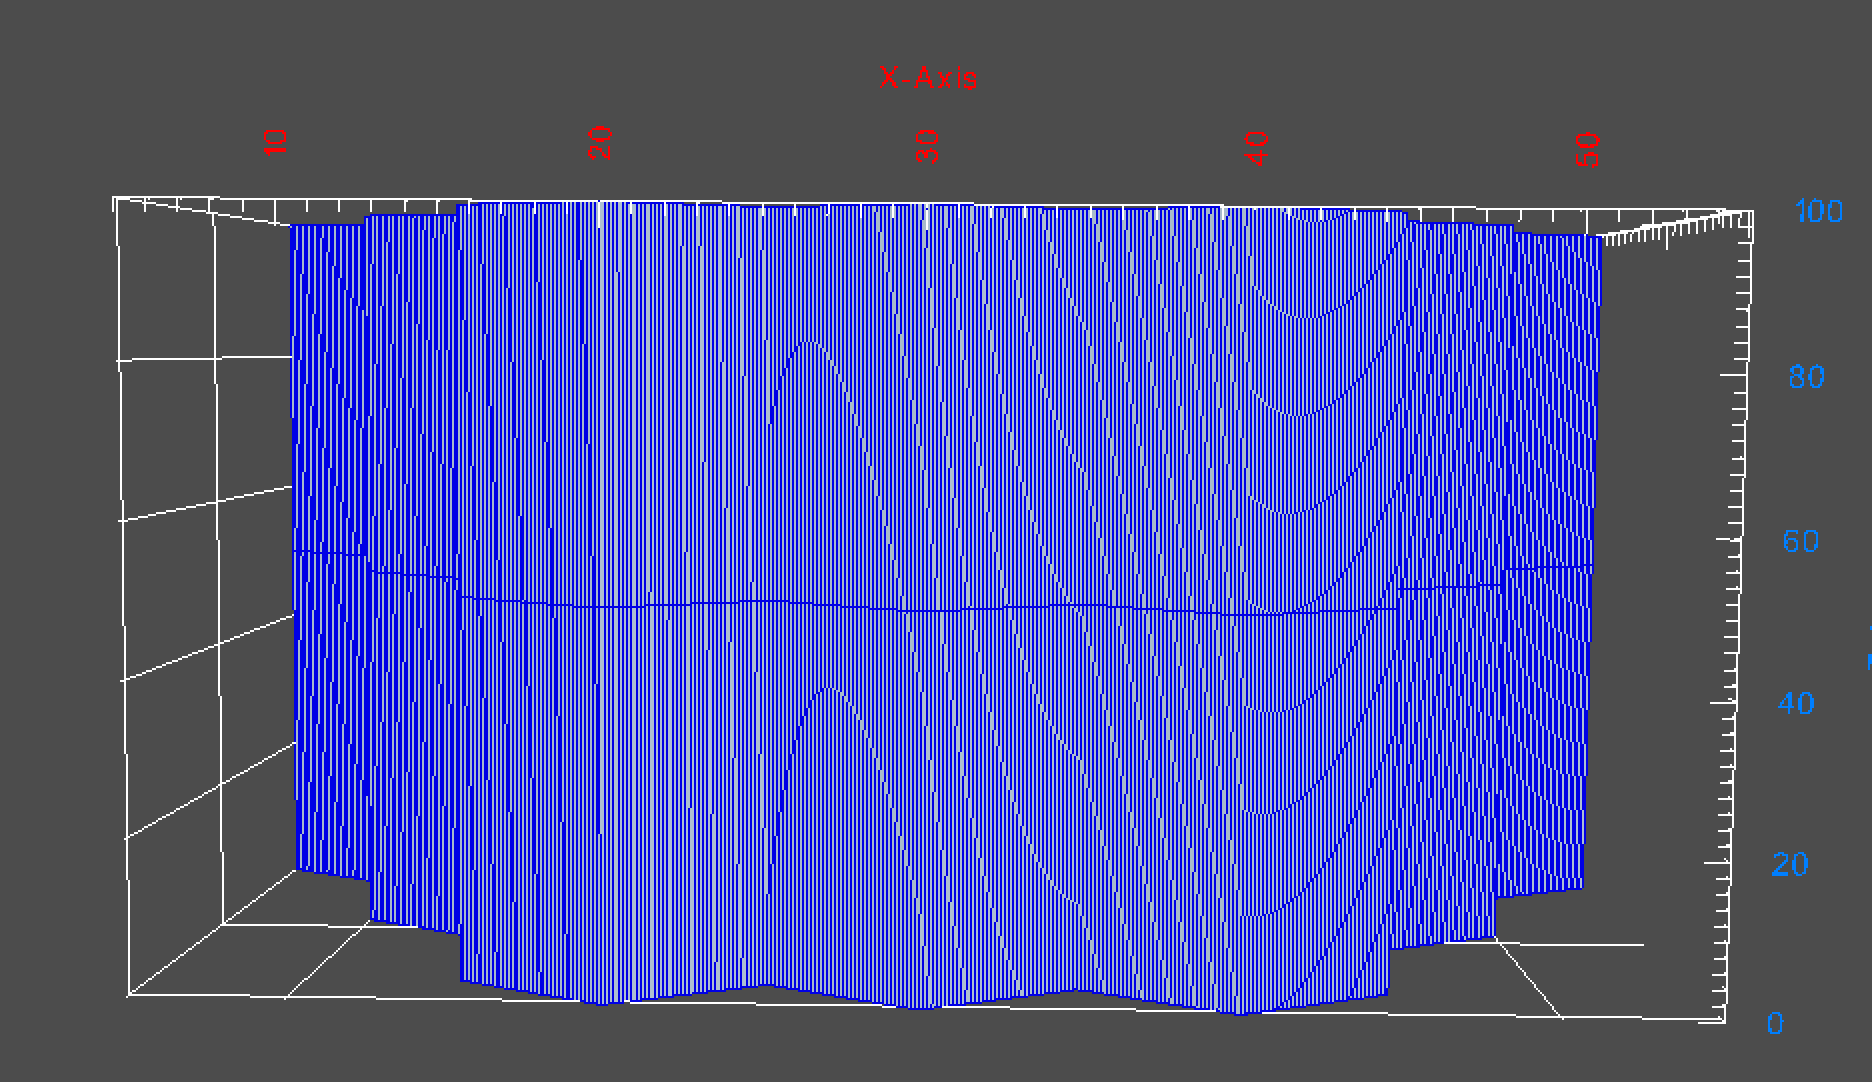
\includegraphics[width=0.5\linewidth]{Images/axial-mesh-50.png}

		\caption{Example of a 100 unit tall core with axial mesh size set to 20 and 50 units.}
		\label{fig:AxialMesh}
	\end{center}
\end{figure}

\toIndex{edge interval}
We also can specify how many edges we'd like along an edge of a hexagonal or rectilinear pin.  We specify this by declaring the edge interval, or the number of mesh edges we'd like per model edge.

\begin{figure}[H]
	\begin{center}
		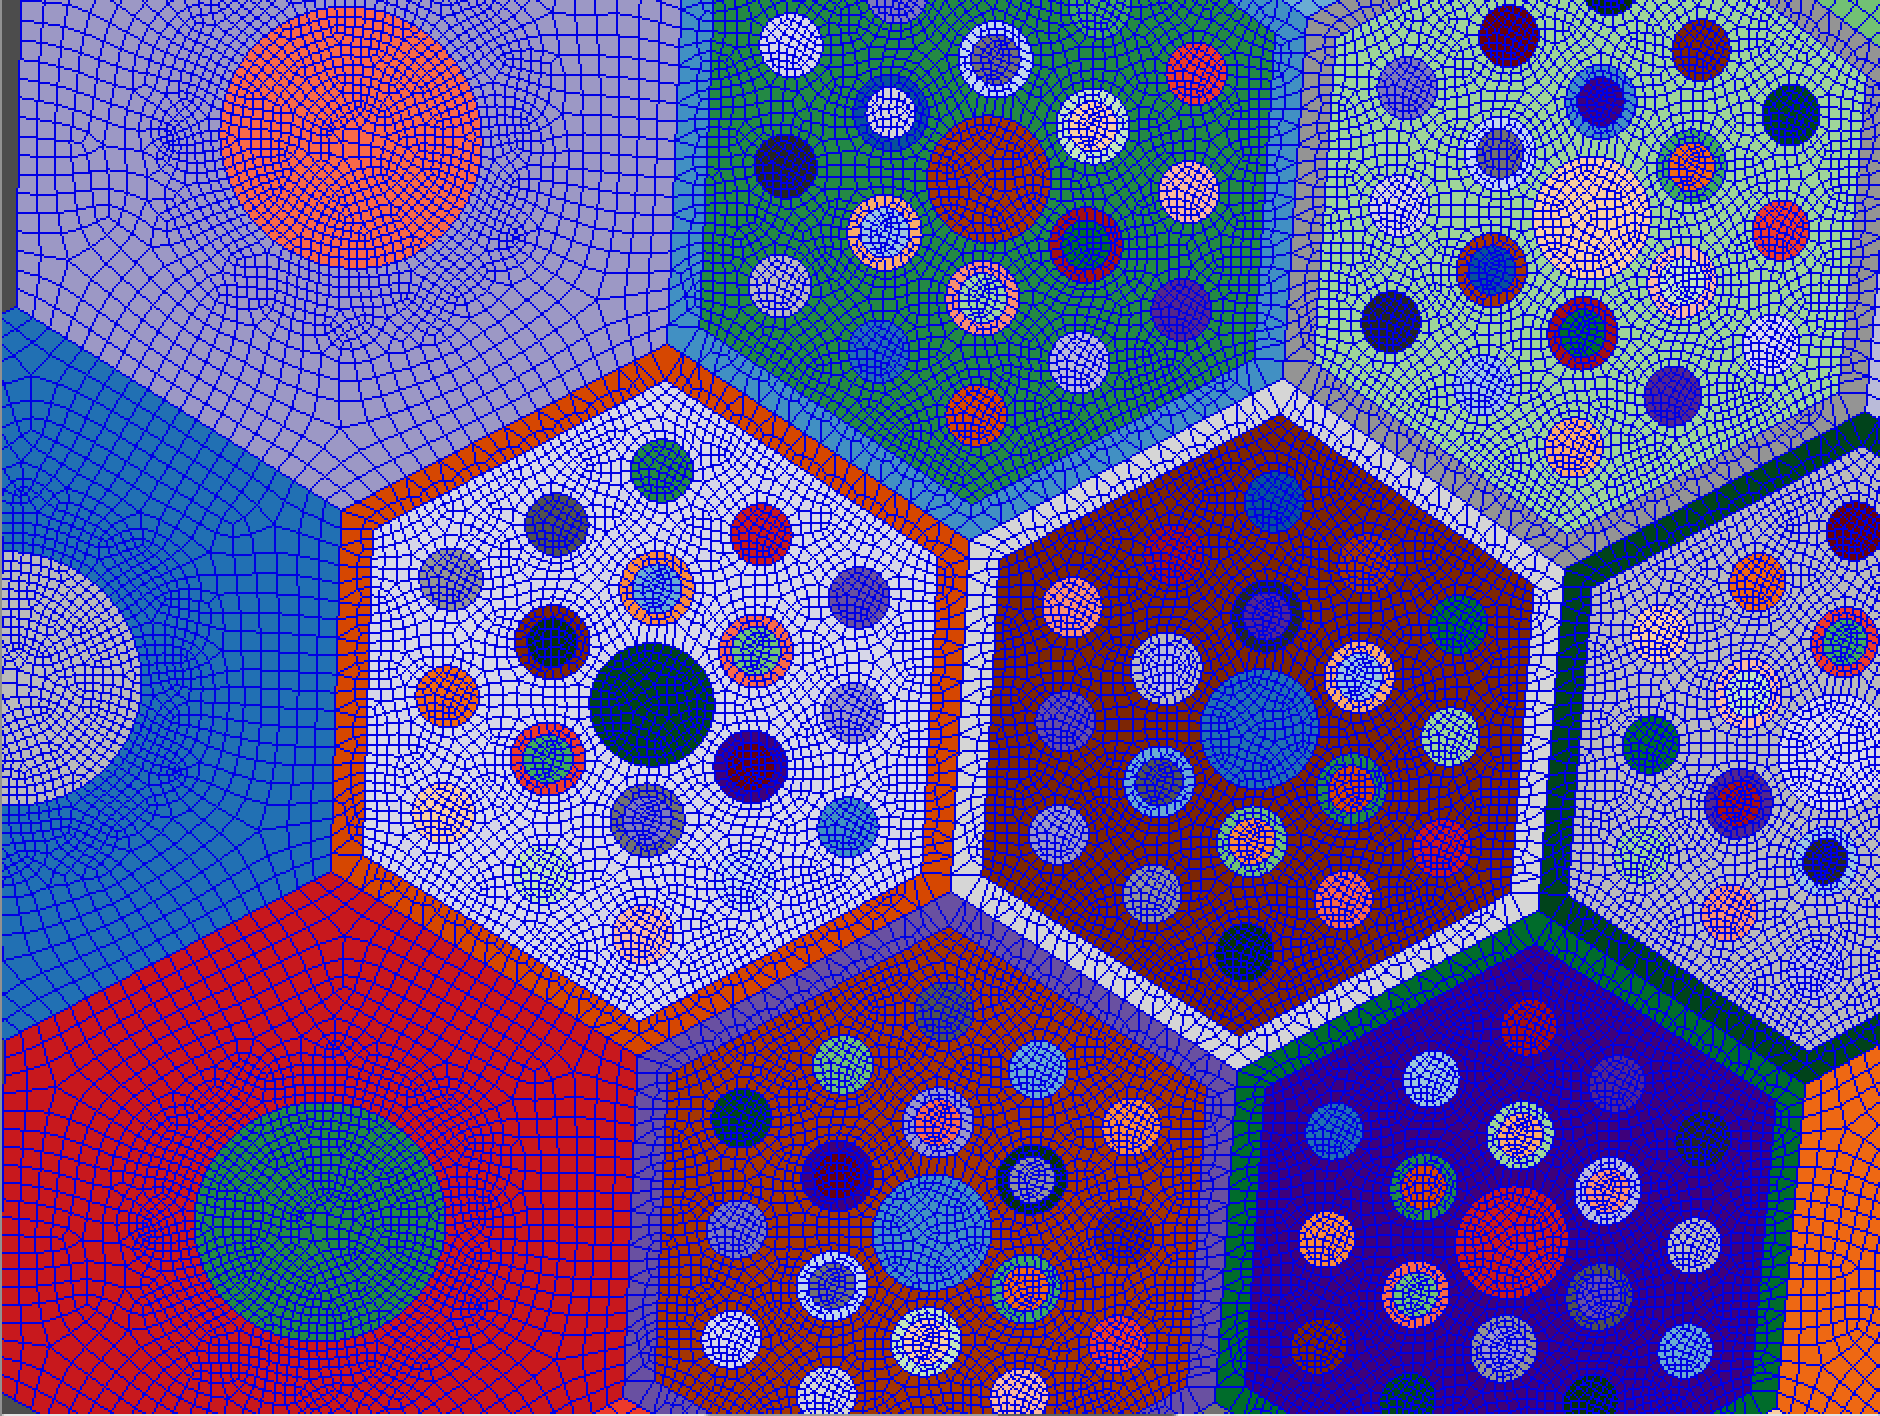
\includegraphics[width=0.5\linewidth]{Images/edge-interval-20.png}
		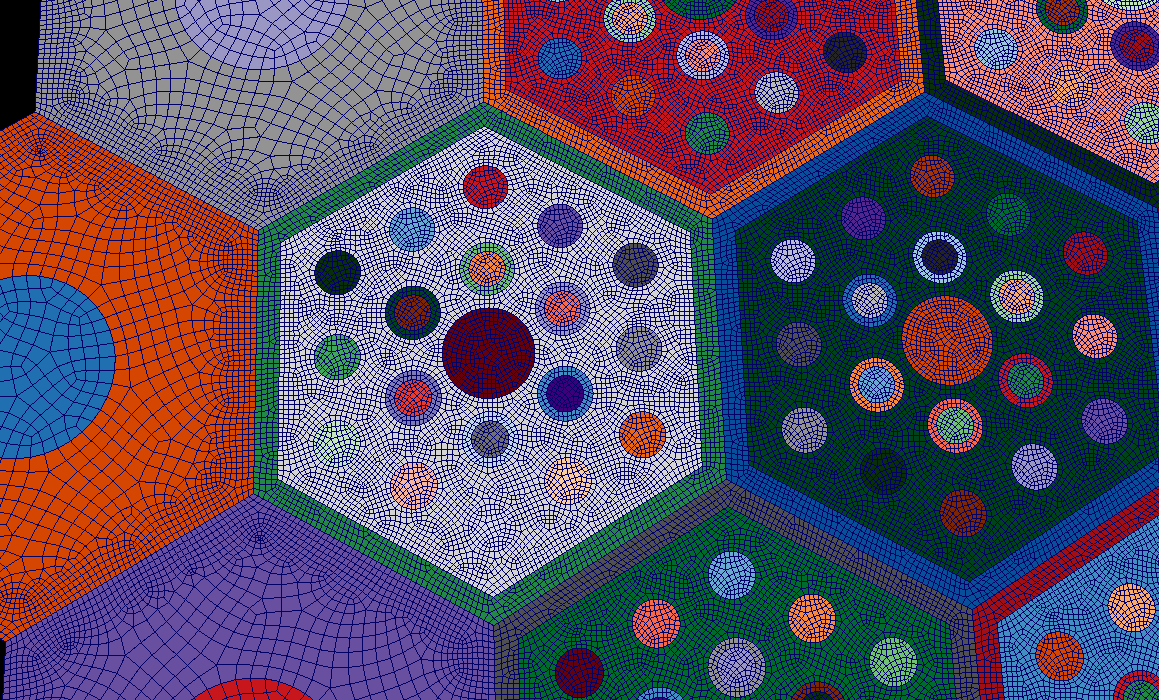
\includegraphics[width=0.5\linewidth]{Images/edge-interval-50.png}

		\caption{Example of a hexagonal core meshes with the edge interval changed.  The top one uses an edge interval of 20 units and the lower one uses an edge interval of 50 units.}
		\label{fig:EdgeInterval}
	\end{center}
\end{figure}

\toIndex{radial mesh size}
\toIndex{mesh size!radial}

\begin{wrapfigure}{r}{0.5\textwidth}
	\begin{center}
		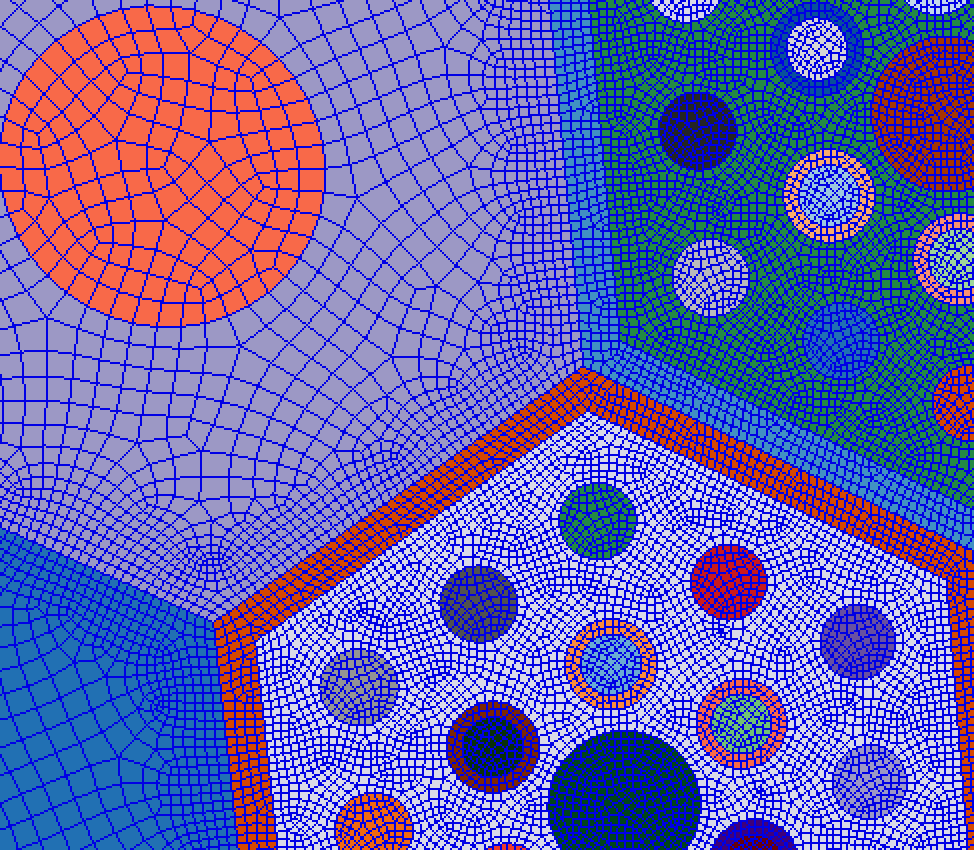
\includegraphics[width=0.8\linewidth]{Images/radial-mesh-size.png}
		\caption{These two assemblies have two different radial mesh sizes.  The one on the left has a radial mesh size of $0.3$, while the one on the right is $0.1$.}
		\label{fig:RadialMesh}
	\end{center}
\end{wrapfigure}

Lastly, we can control how coarse or fine the mesh is by specifying the radial mesh size, or the length of the square or triangle used in the top-down projection of the 3D mesh.  In practice, it does not make sense to choose a radial mesh size larger than the size of the smallest feature you would like to preserve in an assembly, as that would mean that that is not captured in the resulting mesh.

\toIndex{conforming meshes}
\toIndex{meshes!conforming}
Not all meshes are created equal.  Meshes used for analysis must be conforming; that is,

\begin{itemize}
	\item{vertices of mesh polygons or polyhedra must only touch other vertices,}
	\item{edges must only touch other edges,}
	\item{and faces must only contact other mesh faces.}
\end{itemize}

That means that we must ensure that the mesh type, axial mesh size, and edge interval all match in the core.  If they are different in each assembly, the resulting mesh may not always be conforming.  RGG ensures that they match by only letting you specify them at the core level, in the \ui{assembly defaults tab}.

\begin{figure}[H]
	\begin{center}
		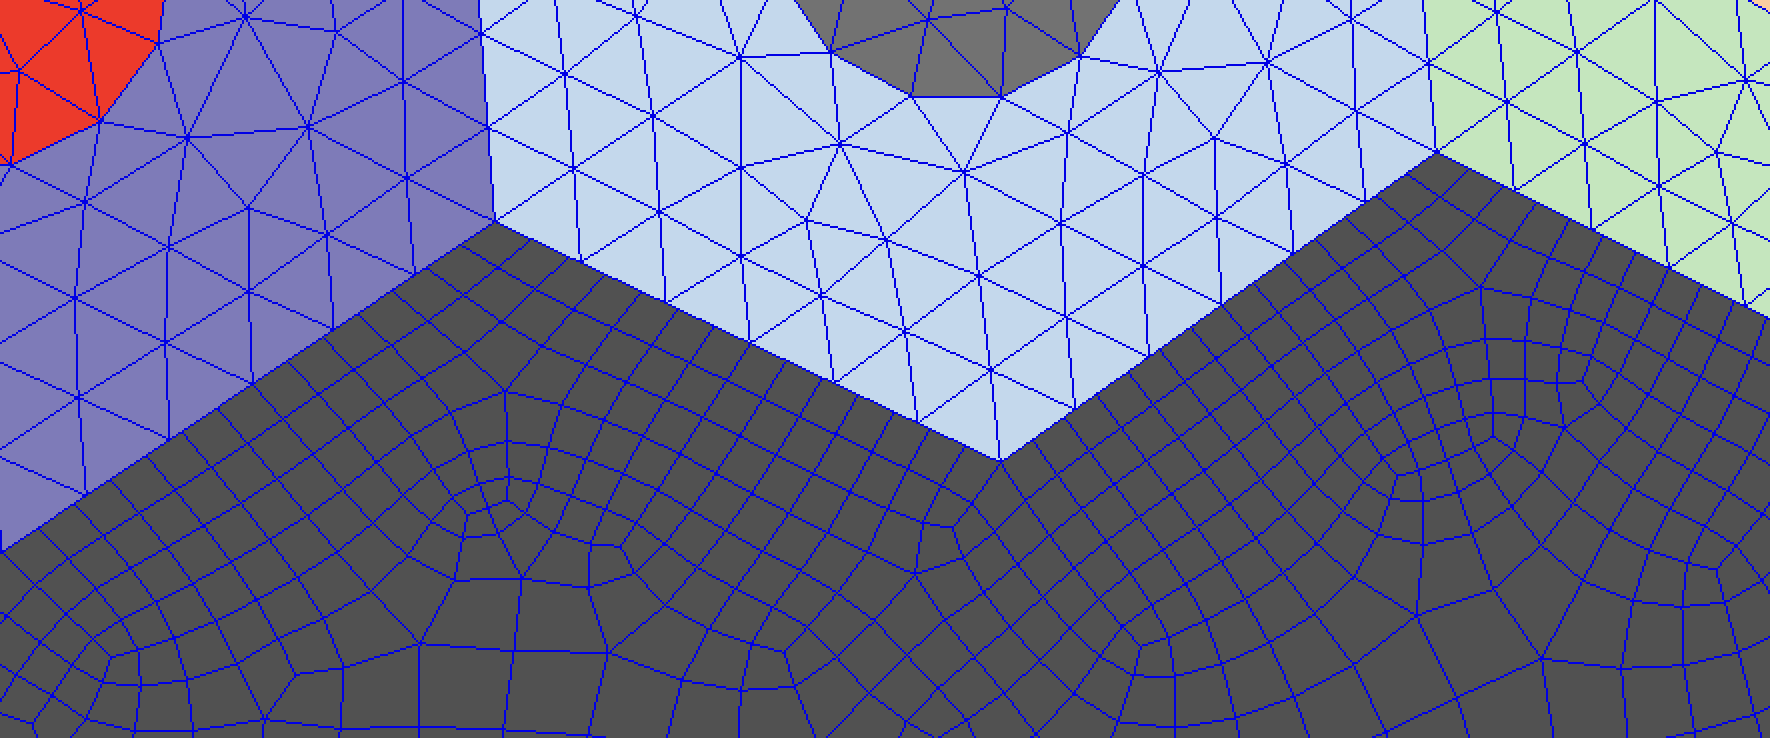
\includegraphics[width=\linewidth]{Images/nonconforming-mesh.png}
		\caption{A non-conforming mesh.  Note how vertices touch edges and edges touch vertices along the border between the blue and the hexes.}
		\label{fig:NonconformingMesh}
	\end{center}
\end{figure}

However, the radial mesh size is not required to be the same for each assembly.  Refer to Figure \ref{fig:RadialMesh}; even though two different assemblies side by side have different radial mesh sizes, it is still conforming. You can change the radial mesh size and specify a different level of coarseness or fineness on a per-assembly basis without suffering bad consequences.  RGG gives you this ability by making radial mesh size accessible from an assembly's \ui{configure tab}.